\documentclass[a4paper, 12pt]{article}
\usepackage[total={17cm,25cm}, top=2.5cm, left=2.5cm, right=2.5cm,  includefoot]{geometry}
\usepackage[utf8]{inputenc}
\usepackage{array}
\usepackage{multirow}
\usepackage{hhline}
\usepackage{gensymb}
\usepackage{graphicx}
\graphicspath{ {} }
\usepackage[czech]{babel}
\usepackage{enumitem}
\usepackage{pdfpages}
\usepackage{amsmath}
\usepackage{verbatim}
\usepackage{listings}
\usepackage{hyperref}
\usepackage{amssymb}


\pagestyle{empty} % vypne číslování stránek




%\usepackage[OT2,OT1]{fontenc}
\newcommand\cyr
{
\renewcommand\rmdefault{wncyr}
\renewcommand\sfdefault{wncyss}
\renewcommand\encodingdefault{OT2}
\normalfont
\selectfont
}
\DeclareTextFontCommand{\textcyr}{\cyr}
\def\cprime{\char"7E }
\def\cdprime{\char"7F }
\def\eoborotnoye{\char’013}
\def\Eoborotnoye{\char’003}


\begin{document}



\begin{titlepage}
\begin{center}
\noindent
\Large \textbf{České vysoké učení technické v Praze }\\ Fakulta stavební
\vspace{5cm}

\huge

%vložení loga cvut
%\begin{figure}[h!]
%	\centering
%	\includegraphics[width=7cm]{logo.png}
%\end{figure}

\vspace{0.5cm}

155ADKG: Digitální model terénu \\

\vspace{10cm}




\Large
Michael Kala\\
Anna Zemánková \\

\end{center}

\end{titlepage}




\pagestyle{plain}     % zapne obyčejné číslování
\setcounter{page}{1}  % nastaví čítač stránek znovu od jedné

%\tableofcontents
%\newpage

\section{Zadání}

\begin{figure}[h!]
	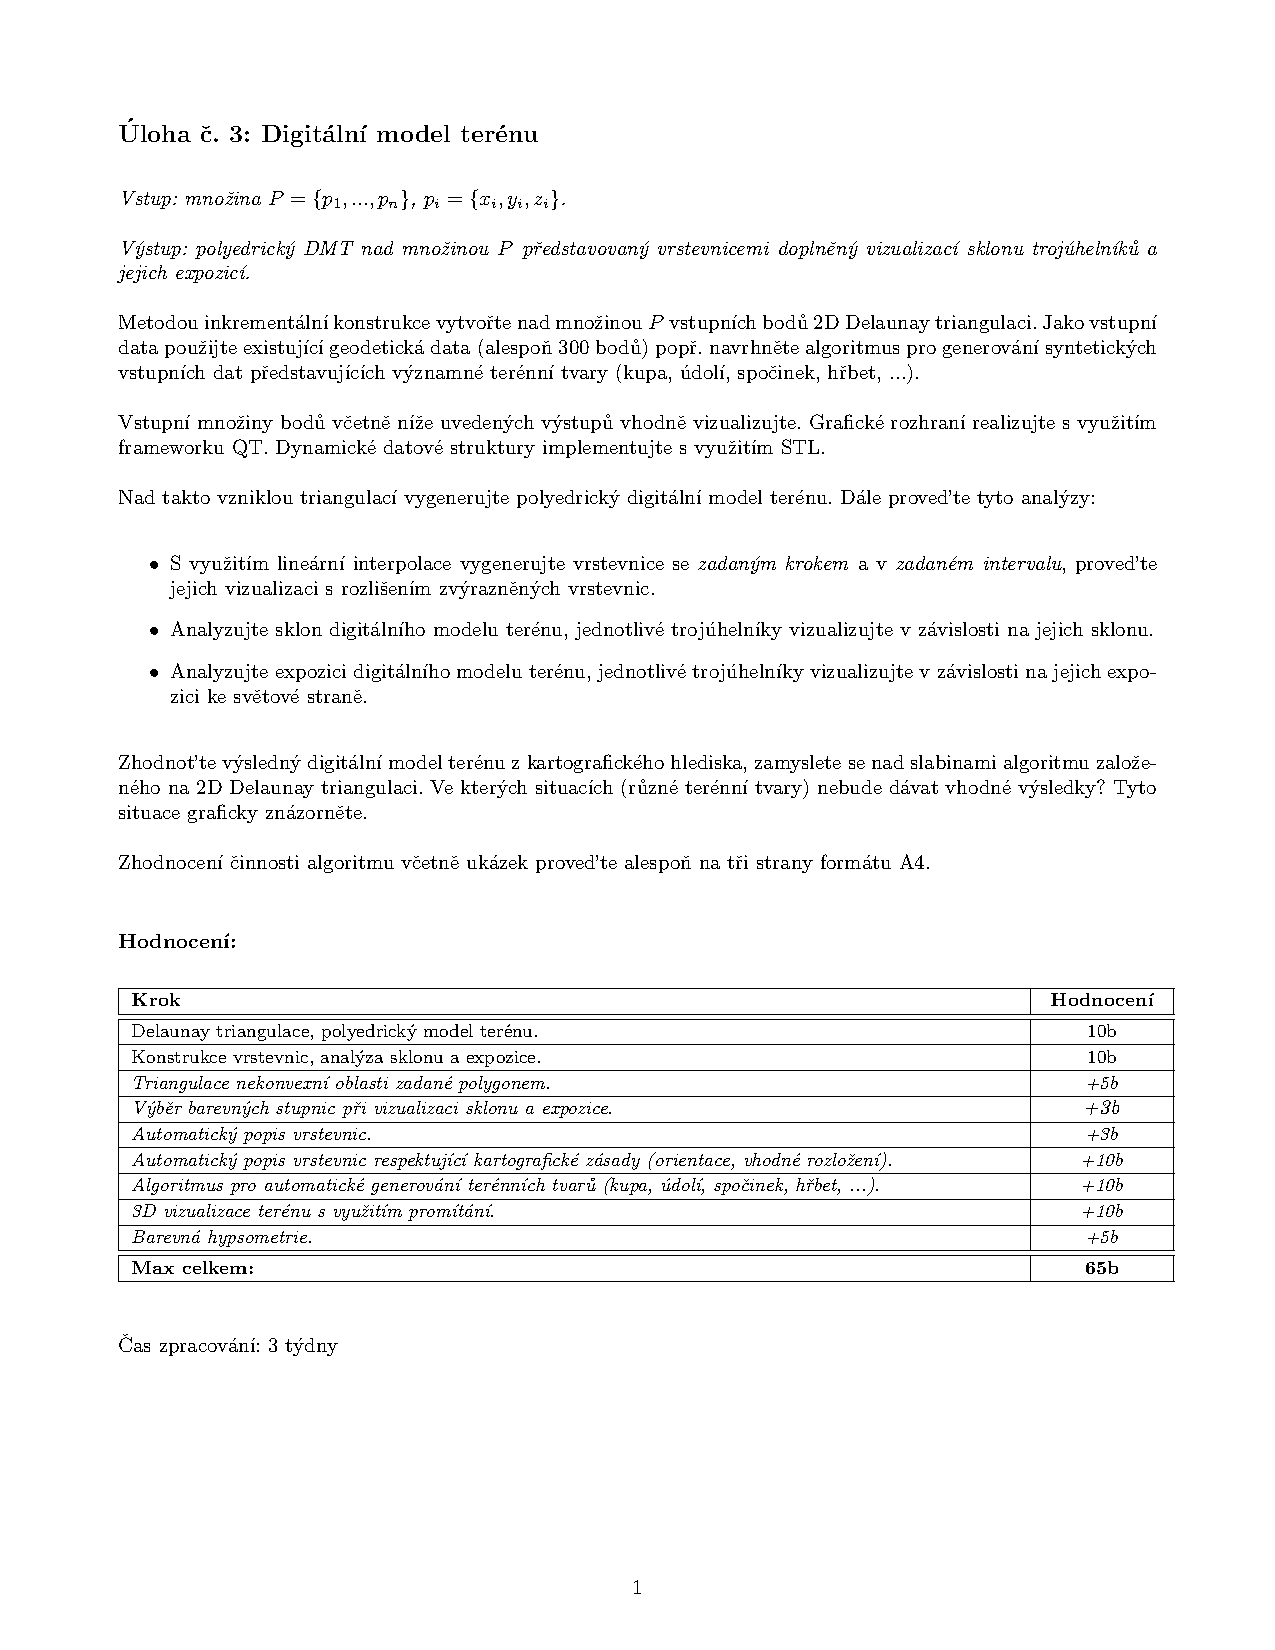
\includegraphics[clip, trim=0cm 5cm 0cm 3cm, width=1.0\textwidth]{zadani.pdf}
\end{figure}


\section{Údaje o bonusových úlohách}
Z bonusových úloh byly zpracovány:
\begin{itemize}
	\item automatický popis vrstevnic
	\item barevná hypsometrie
\end{itemize}



\clearpage

\section{Popis a rozbor problému}

Mějme množinu bodů $P \{p_i\}$,  $p_i = \{x_i, y_i, z_i\}$. Nad touto množinou chceme vytvořit síť trojúhelníků $t_j$ pomocí Delaunay triangulace $DT$, následně vytvořit vrstevnice a pro vizualizaci DMT určit sklon a expozici jednotlivých trojúhelníků.\\ 

\subsection{Delaunay triangulace}
Vlastnosti:
\begin{itemize}
\item Uvnitř kružnice opsané trojúhelníku $t_j \in DT$ neleží žádný jiný bod množiny P.
\item $DT$ maximalizuje minimální úhel v $\forall t_j$, avšak $DT$ neminimalizuje maximální úhel v $t_j$.
\item $DT$ je lokálně optimální i globálně optimální vůči kritériu minimálního úhlu.
\item $DT$ je jednoznačná, pokud žádné čtyři body neleží na kružnici.
\end{itemize}
\vspace{1.5cm}

\subsection{Vrstevnice}
Vrstevnice byly určeny za využití lineární interpolace, při které se předpokládá, že spád terénu je mezi podrobnými body $p_i$, mezi nimiž se provádí interpolace, konstantní.\\

Mějme trojúhelník $t_j$, tvořený hranami $e_1, e_2, e_3$ a rovinu vrstevnice $\rho$ o dané výšce.

Vztah hrany tojúhelníku a roviny vrstevnice:
\begin{enumerate}
\item $(z-z_i)*(z-z_{i+1}) < 0$  $\longrightarrow e_i \cap \rho$
\item $(z-z_i)*(z-z_{i+1}) > 0$  $\longrightarrow e_i \notin \rho$ 
\item $(z-z_i)*(z-z_{i+1}) = 0$  $\longrightarrow e_i \in \rho$
\end{enumerate}

\noindent Pokud  $e_1, e_2, e_3 \in \rho$, jedná se o trojúhelník náležící rovině $\rho$ a není nutné vrstevnici pro tento trojúhelník řešit.\\
Jestliže $e_i \cap \rho$, je vypočten průsečík hrany $e_i = (p_1, p_2)$ a roviny vrstevnice $\rho$ o výšce $z$:
$$ x = \frac{(x_2-x_1)}{(z_2-z_1)}(z-z_1)+x_1, $$
$$ y = \frac{(y_2-y_1)}{(z_2-z_1)}(z-z_1)+y_1.$$
\clearpage

\subsection{Sklon}

Sklon je úhel $\varphi$ mezi svislicí $n$ a normálou trojúhelníku $n_t$. Rovina trojúhelníku $t_j$ je určena vektory u,v.\\

\noindent $$n = (0,0,1)$$
$n_t = \vec{u}\times \vec{v}$
$$\varphi =\arccos(\frac{n_t \cdot n}{|n_t| |n|})$$
\\
Sklon je vizualizován odstíny šedi.


\subsection{Expozice}
Expozice je orientace trojúhelníku vůči světovým stranám.\\
$$A = \arctan2(\frac{n_x}{n_y});$$ kde $n_x, n_y$ jsou vektorové součiny $u$ a $v$.\\

\noindent Expozice je vizualizována pomocí barevného spektra, barvy byly vybrány stejně jako v SW ArcMAP - ESRI:\\
\begin{figure}[h]
	\centering
	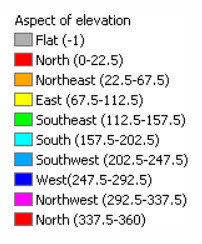
\includegraphics[width=4cm]{expozice.jpg}
	\caption{Vizualizace expozice}
\end{figure}


\clearpage
\section{Popis algoritmů}

\subsection{Delaunayova triangulace}
Triangulace byla realizována metodou inkrementální konstrukce, body jsou tedy do triangulace přidávány postupně a to tak, aby vybraný bod ležel v levé polorovině od orientované hrany, poloměr opsané kružnice byl minimální a zároveň jsou preferovány body, jejichž střed opsané kružnice leží v pravé polorovině. Pokud žádný bod těmto kritériím nevyhovuje, je orientace hrany obrácena a bod je vybírán znovu. Jakmile je bod nalezen, jsou k němu vytvořeny orientované hrany a vše je uloženo do triangulace.\\
Pro "manipulaci" s hranami se používá struktura Active Edges List $AEL$, do ní jsou ukládány hrany, ke kterým je třeba nalézt třetí bod a vytvořit trojúhelník. Jakmile je $AEL$ prázdná, algoritmus končí.

\subsubsection{Implementace metody}
\begin{enumerate}
\item $ p_1 = rand(P), ||p_2-p_1|| = min $ ....náhodný a nebližší bod
\item Vytvoř hranu $ e = (p_1,p_2) $ 
\item Inicializuj: $p_{min} = arg min_{\forall p_i\in\sigma_L(e)} r'(k_i), k_i = (a, b, p_i), e = (a,b)$
\item Pokud $ \nexists p_{min},$ prohoď orientaci $e \longleftarrow (b,a) $. Jdi na $3)$
\item $e_2 = (p_1,p_{min}), e_3 = (p_{min},p_1) $...zbývající hrany trojúhelníku
\item $AEL \longleftarrow e, AEL \longleftarrow e_2, AEL \longleftarrow e_3 $
\item $DT \longleftarrow e, DT \longleftarrow e_2, DT \longleftarrow e_3 $ 
\item while AEL not empty:
\item \hspace {1cm} $AEL  \longrightarrow e, e = (p_1, p_2) $....vezme první hranu z AEL
\item \hspace {1cm}$ e = (p_2, p_1)$ ...prohodí její orientaci
\item \hspace {1cm} $p_{min} = arg min_{\forall p_i\in\sigma_L(e)} r'(k_i), k_i = (a, b, p_i), e = (a,b) $
\item \hspace {1cm} if $ \exists p_{min}:$
\item \hspace {2cm} $e_2 = (p_1,p_{min}), e_2 = (p_{min},p_1) $...zbývající hrany trojúhelníku
\item \hspace {2cm} $DT \longleftarrow e  $  
\item \hspace {2cm} $ add(e_2,AEL,DT), add(e_3,AEL,DT)$
\end{enumerate}
\clearpage
Dílčí algoritmus Add:
\begin{enumerate}
	\item Vytvoř hranu $e' = (b,a)$
	\item if $(e' \in AEL)$
	\item \hspace {1cm} $ AEL \longrightarrow e'$...Odstraň z AEL
	\item else:
	\item \hspace {1cm} $ AEL \longleftarrow e$ ...Přidej do AEL
	\item $DT\longleftarrow (a,b)$ Přidej do DT
\end{enumerate}


\subsection{Barevná hypsometrie}
Myšlenka výpočtu barevné hypsometrie vychází z procházení všech trojúhelníků triangulace i s jejich vrstevnicemi. Výpočet pak vždy probíhá nad jedním trojúhelníkem. Jediný moment při běhu programu, kdy lze získat trojúhelníky a jejich vrstevnice dohromady, je při výpočtu vrstevnic. Proto výpočet hypsometrie probíhá zároveň s výpočtem vrstevnic. Samostatný algoritmus vypadá následovně:

\begin{enumerate}
	\item Vytvoř vektor polygonů \textbf{pols} s údajem o jejich střední výšce
	\item Procházej po jednom všechny trojúhelníky:
		\begin{enumerate}
			\item Do vektoru bodů \textbf{pts} ulož vrcholy trojúhelníku a krajní body vrstevnic
			\item Vytvoř vektor vektorů bodů \textbf{vec\_pts} o velikosti počtu intervalů vrstevnic v rámci trojúhelníku (počítají se i krajní intervaly, ve kterých může ležet vrchol trojúhelníku)
			\item Procházej vektor bodů \textbf{pts} a ulož body podle výšky do příslušného vektoru bodů z \textbf{vec\_pts}.
			\item Vypočítej konvexní obálku každého vektoru bodů z \textbf{vec\_pts}, vypočti jejich průměrnou výšku a ulož do \textbf{pols}. 
		\end{enumerate}
	\item Seřaď \textbf{pols} bodle středních výšek.
	\item Naškáluj tabulku barev podle počtu polygonů v \textbf{pols}.
	\item Vykresli polygony.
\end{enumerate}

Pozn.: Pro vytvoření polygonů bylo třeba každou množinu bodů seřadit tak, aby byly ve správném pořadí. K tomu byl využit algoritmus Sweep Line z minulé úlohy (možná dělo na vrabce, ale funkční a již ověřené).

\subsection{Automatický popis vrstevnic}
Při vytváření vrstevnic je zároveň ukládána jejich výška. Vektor výšek je pak procházen společně s vektorem vrstevnic a ke každé hlavní je přidán popisek.

\clearpage

% ===============================================================

\section{Vstupní data}

Vstupními daty je textový soubor \textit{*.txt} se souřadnicemi bodů ve tvaru [X,Y,Z]. Lze jej do aplikace nahrát pomocí tlačítka \textit{Load points}.\\

\noindent Součástí příloh je textový soubor s testovacími daty \textit{testovaci\_data.txt}.

\vspace{4.5cm}

\section{Výstupní data}
Výsledky aplikace jsou vizualizovány v kanvasu grafického rozhraní.

%OBRÁZEK
\begin{figure}[h]
	\centering
	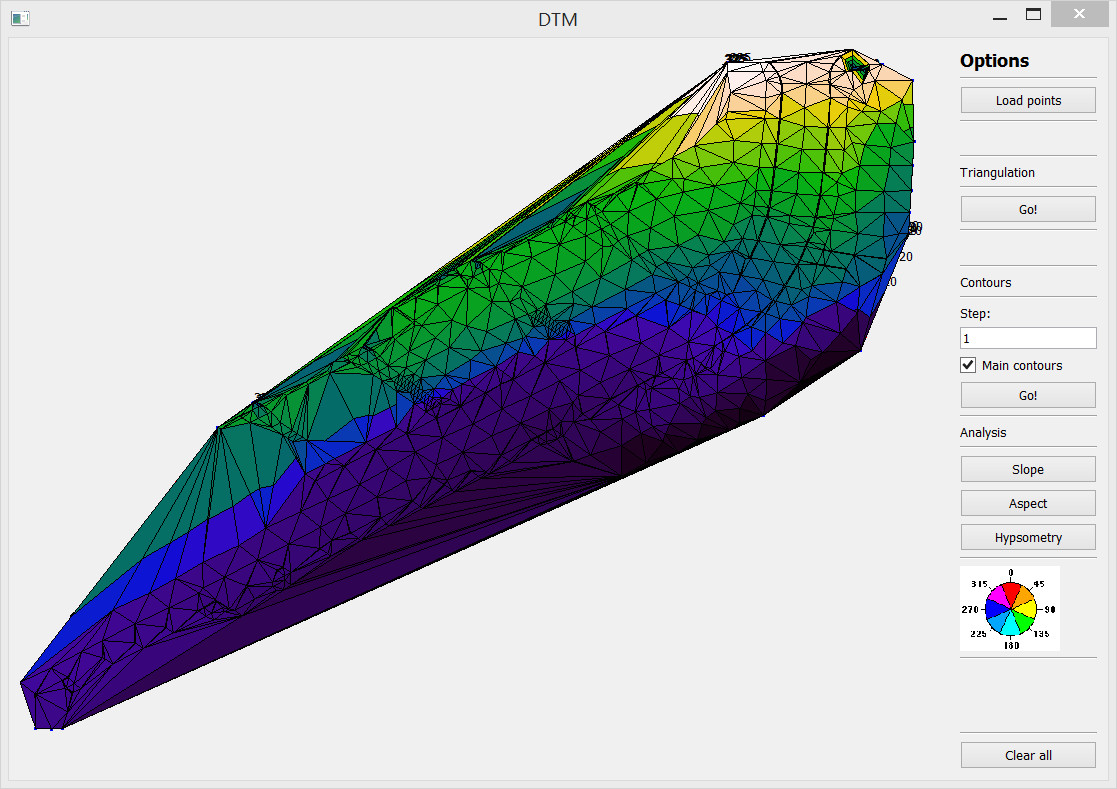
\includegraphics[width=10cm]{hypsometrie.jpg}
	\caption{Výstup}
\end{figure}

\clearpage

\section{Ukázka vytvořené aplikace}


%OBRÁZEK
\begin{figure}[h]
	\centering
	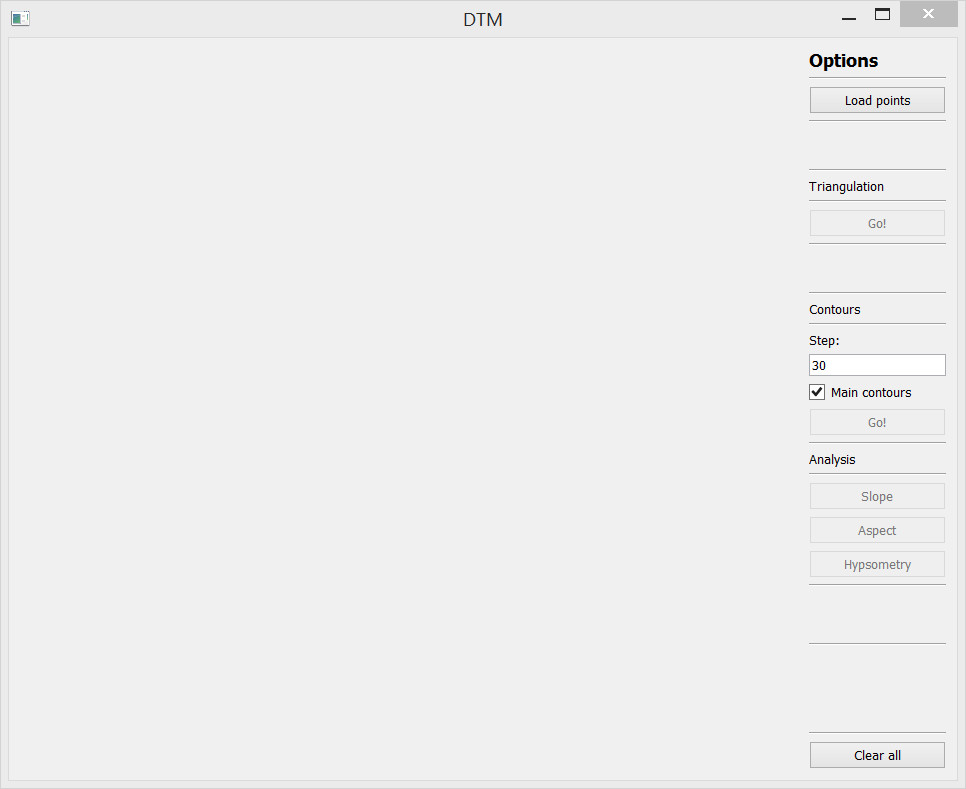
\includegraphics[width=10cm]{aplikace.jpg}
	\caption{Rozvržení aplikace}
\end{figure}

Nejprve je třeba nahrát vstupní data pomocí tlačítka \textit{Load points} a následně je možné vypočítat Delaunay triangulaci, teprve poté jsou zpřístupněna i ostatní tlačítka aplikace kromě barevné hypsometrie. \\

%OBRÁZEK
\begin{figure}[h]
	\centering
	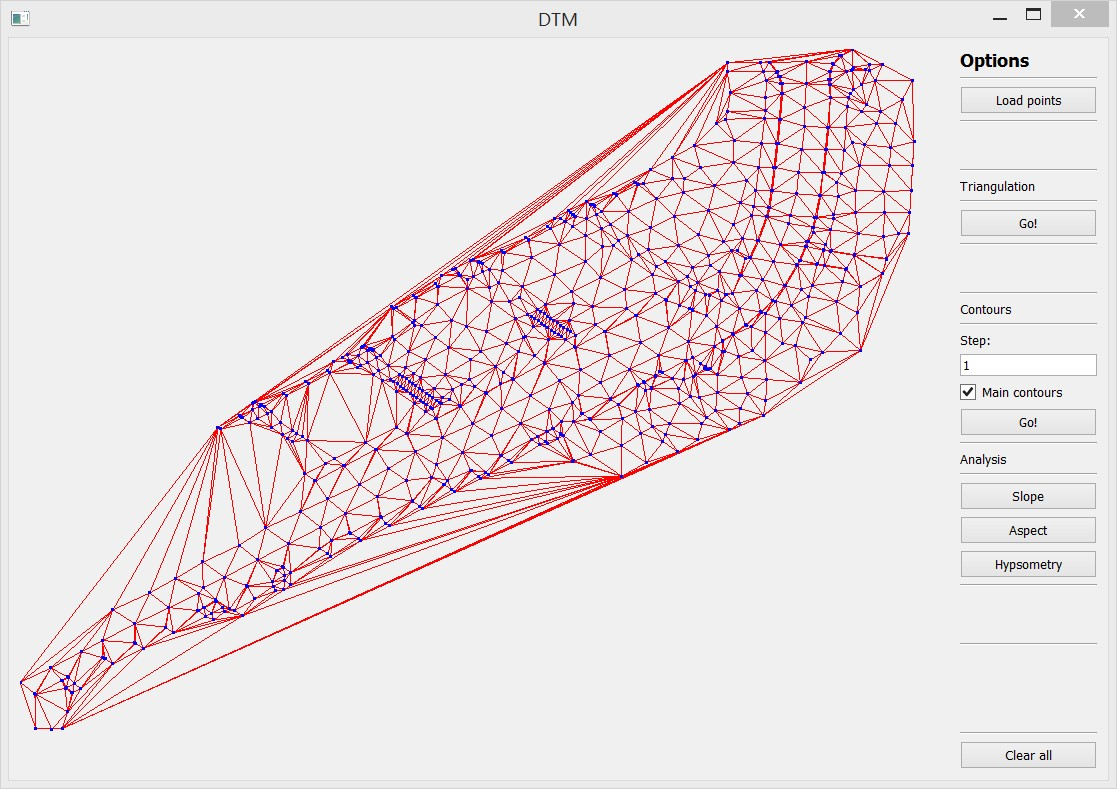
\includegraphics[width=10cm]{DT.jpg}
	\caption{Delaunay triangulace}
\end{figure}

\clearpage

Při výpočtu vrstevnic je třeba zadat krok vrstevnic a (ne)zaškrtnout zvýraznění hlavních vrstevnic. Po výpočtu vrstevnic je zpřístupněno tlačítko pro barevnou hypsometrii.

%OBRÁZEK
\begin{figure}[h]
	\centering
	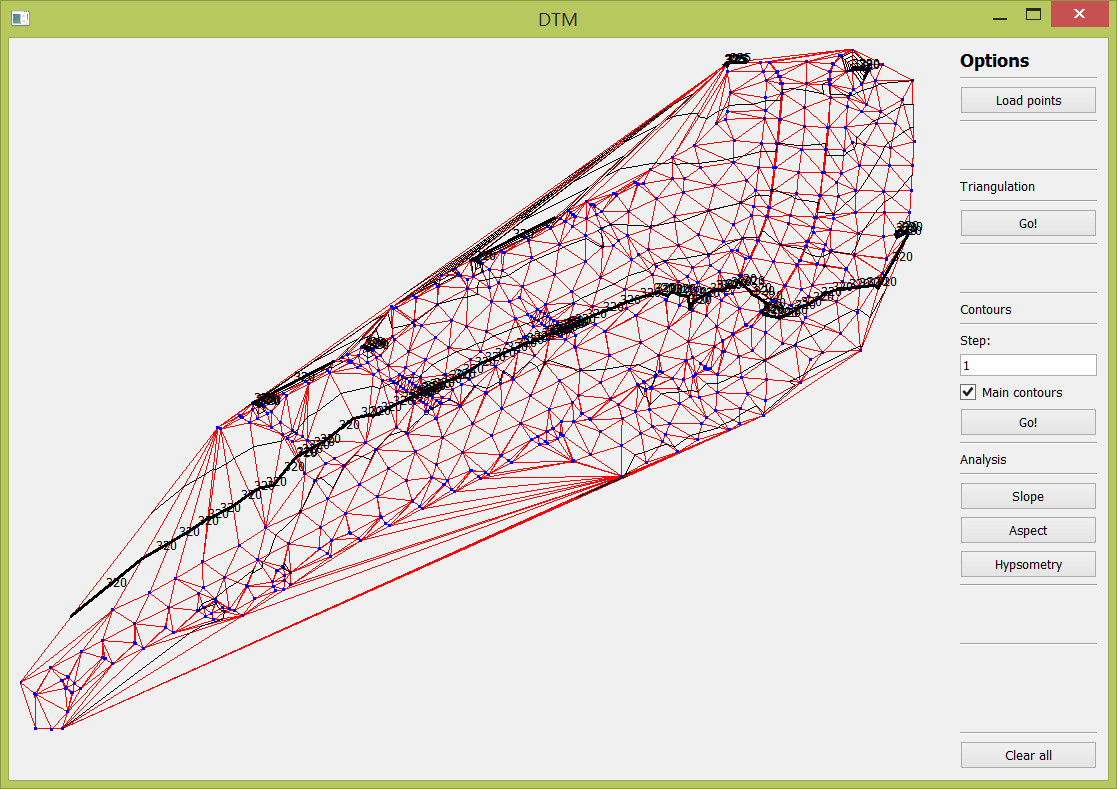
\includegraphics[width=10cm]{vrstevnice.jpg}
	\caption{Vrstevnice}
\end{figure}

V sekci analysis je možné vypočíst a vizualizovat sklon a expozici či barevnou hypsometrii. Po opětovném stisknutí příslušného tlačítka se daná vizualizace opět skryje.
%OBRÁZEK
\begin{figure}[h]
	\centering
	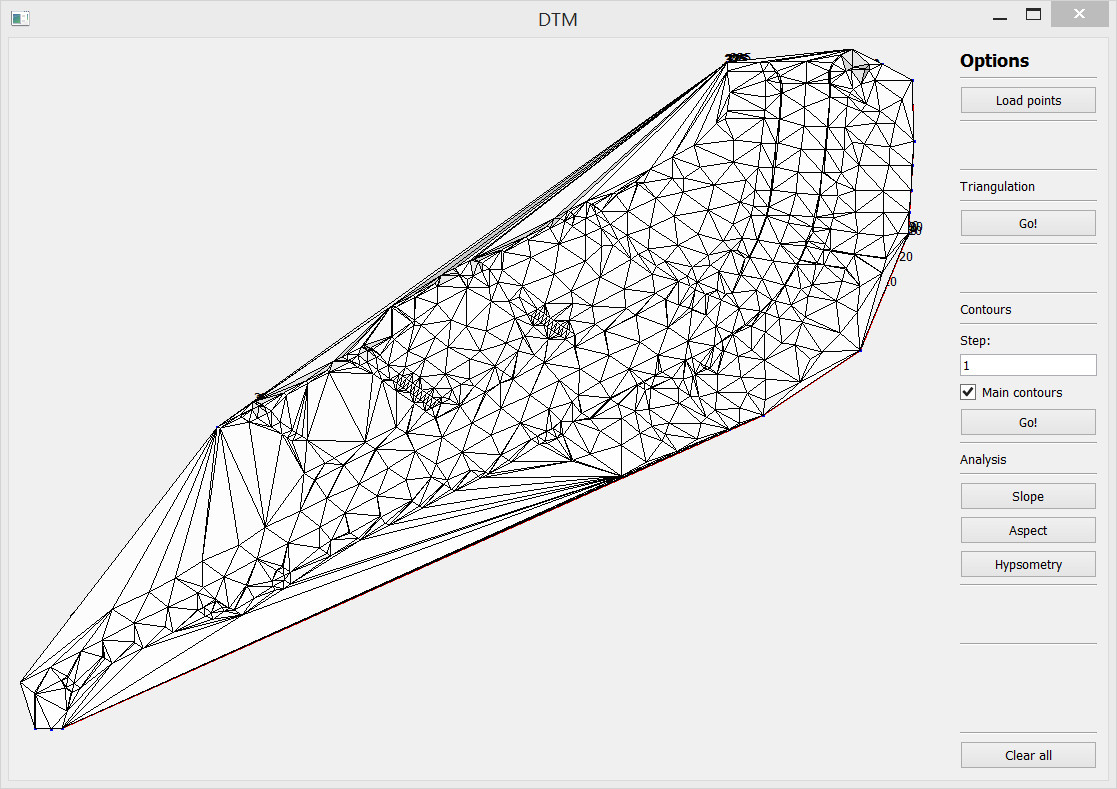
\includegraphics[width=10cm]{sklon.jpg}
	\caption{Sklon}
\end{figure}

\clearpage

%OBRÁZEK
\begin{figure}[h]
	\centering
	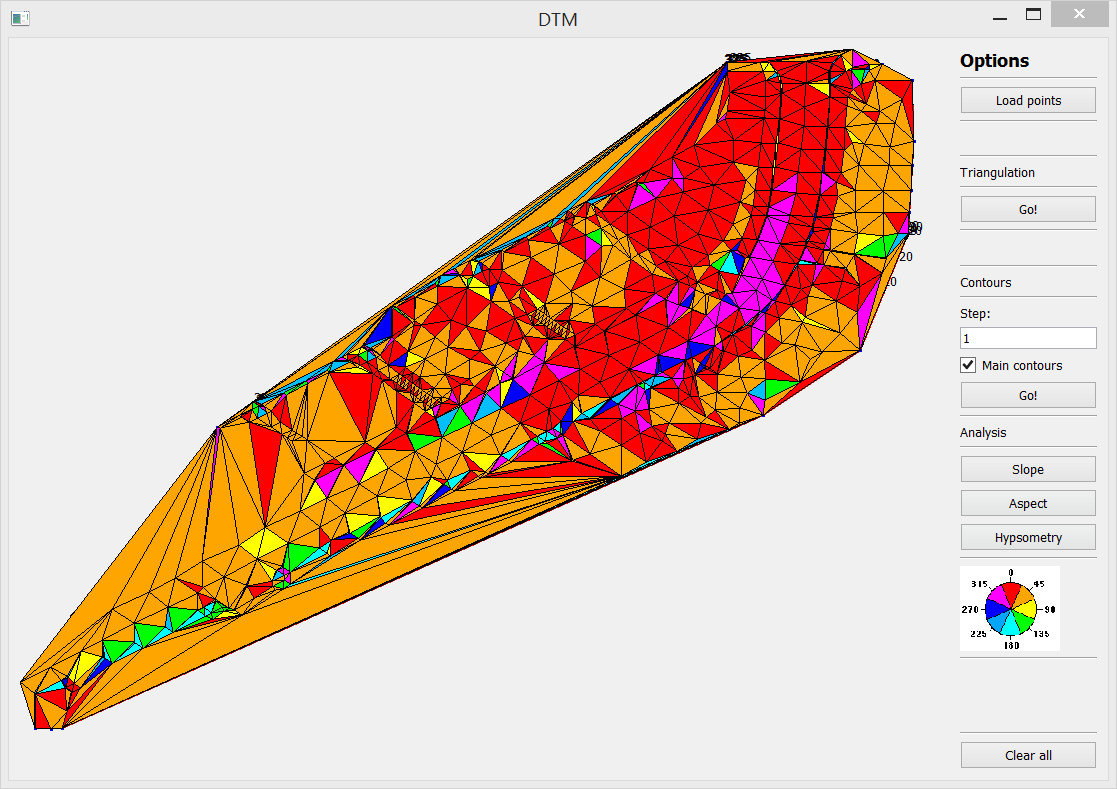
\includegraphics[width=10cm]{aspect.jpg}
	\caption{Expozice}
\end{figure}

%OBRÁZEK
\begin{figure}[h]
	\centering
	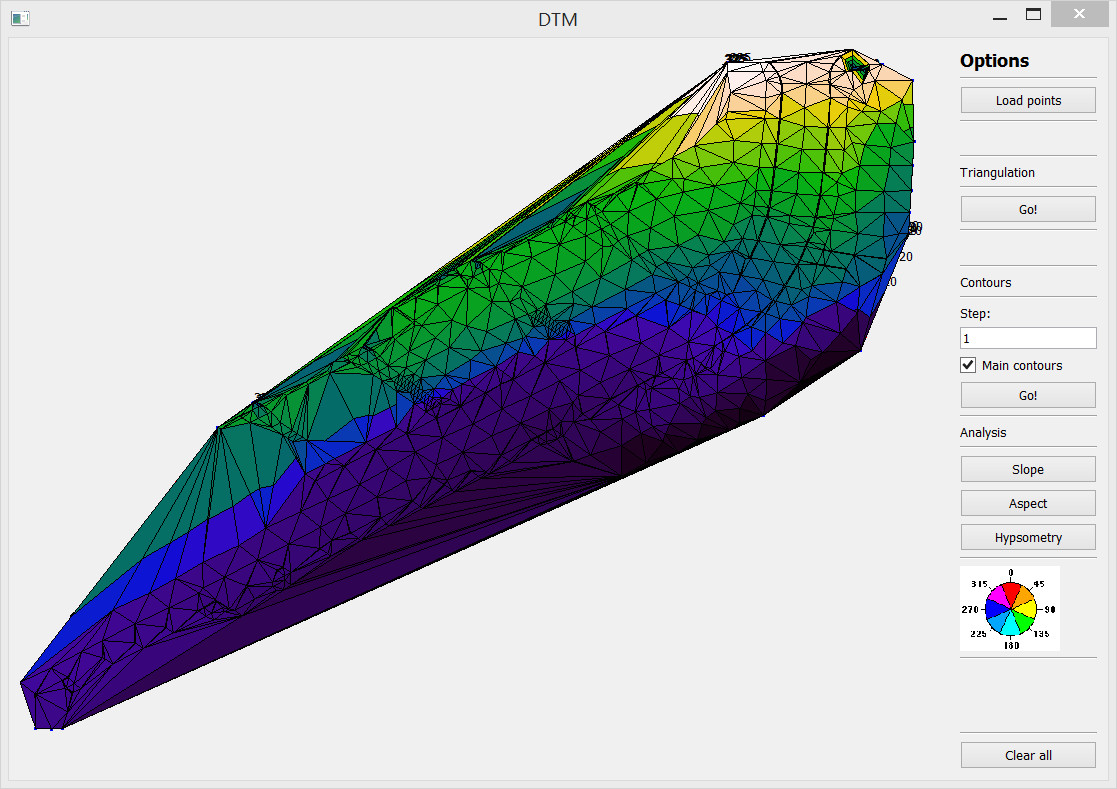
\includegraphics[width=10cm]{hypsometrie.jpg}
	\caption{Barevná hypsometrie}
\end{figure}


Vše je uvedeno do původního stavu (smazány body i vypočtené výsledky) kliknutím na tlačítko Clear.\\
\clearpage

\section{Zhodnocení algoritmu}

Na obrázcích níže je porovnán DMT vyhotovený v SW Atlas se zadáváním povinných hran a DMT vytvořený v naší aplikaci.\\


\textbf{Kráter}\\
Terénní útvar s pracovním názvem kráter je DT poměrně hezky vystižen především s pomocí vrtevnic, samotný DMT bez vrstevnic už tak názorný není.
 
\begin{figure}[h]
	\centering
	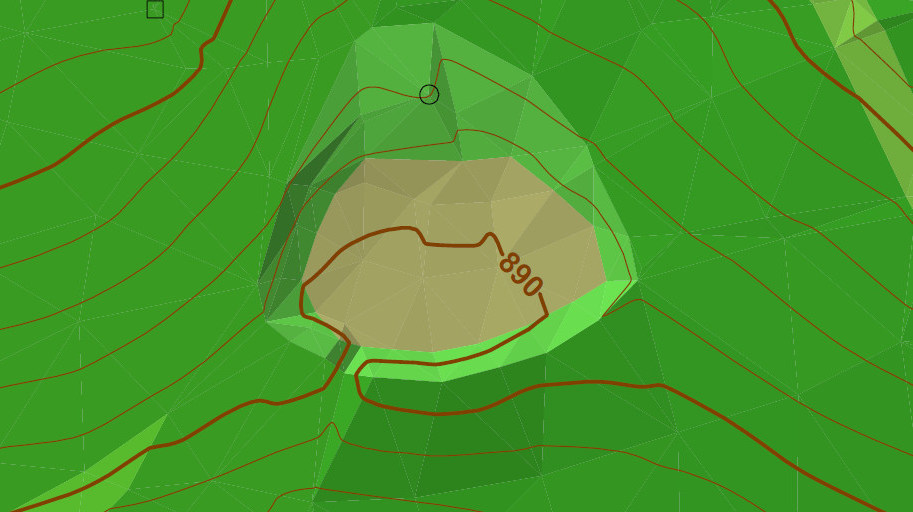
\includegraphics[width=8.5cm]{krater.jpg}
	\caption{kráter - Atlas}
\end{figure}

\begin{figure}[h]
	\centering
	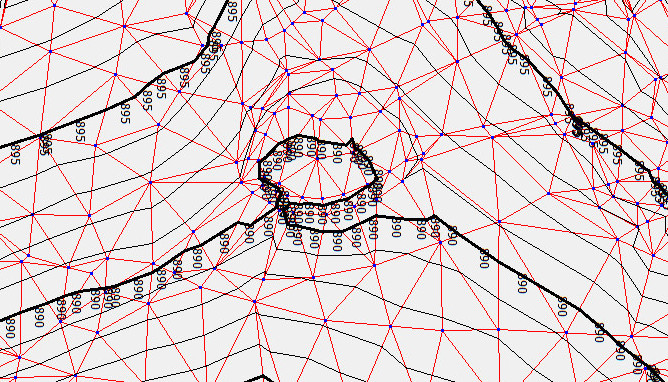
\includegraphics[width=8.5cm]{krater_nas.jpg}
	\caption{kráter - vrstevnice}
\end{figure}

\begin{figure}[h]
	\centering
	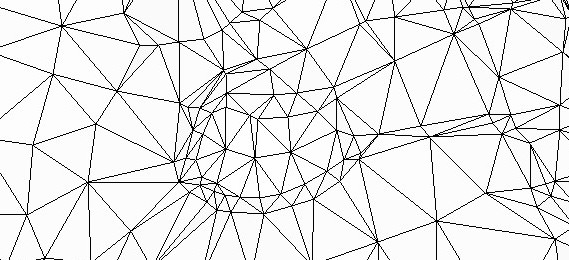
\includegraphics[width=8.5cm]{krater_nas2.jpg}
	\caption{kráter}
\end{figure}
\clearpage

\textbf{Hrana silnice}

Výrazná hrana - okraj silnice je místy kostrbatá - bylo by třeba ji zadat jako povinnou.

\begin{figure}[h]
	\centering
	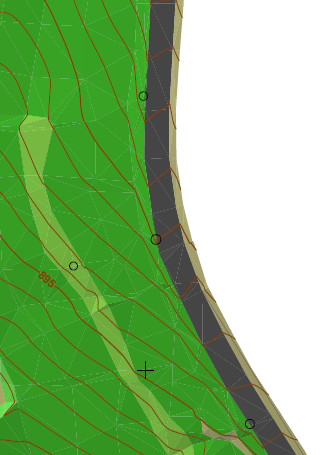
\includegraphics[width=5cm]{hrana_atlas.jpg}
	\caption{Hrana - Atlas}
\end{figure}

\begin{figure}[h]
	\centering
	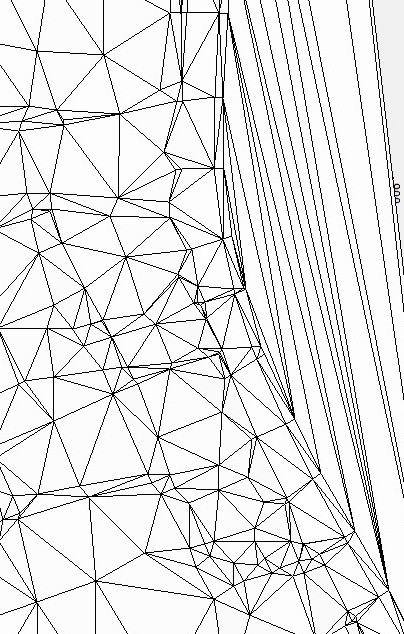
\includegraphics[width=5cm]{hrana_nase.jpg}
	\caption{Hrana}
\end{figure}

\clearpage

\textbf{Údolnice}
\begin{figure}[h]
	\centering
	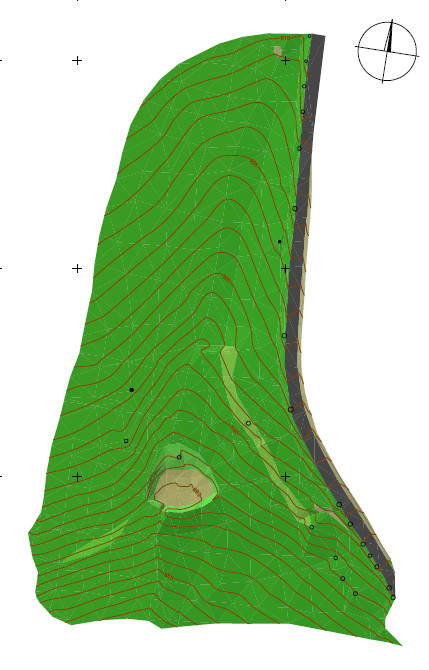
\includegraphics[width=10cm]{dmt_atlas.jpg}
	\caption{Údolnice - Atlas}
\end{figure}

\begin{figure}[h]
	\centering
	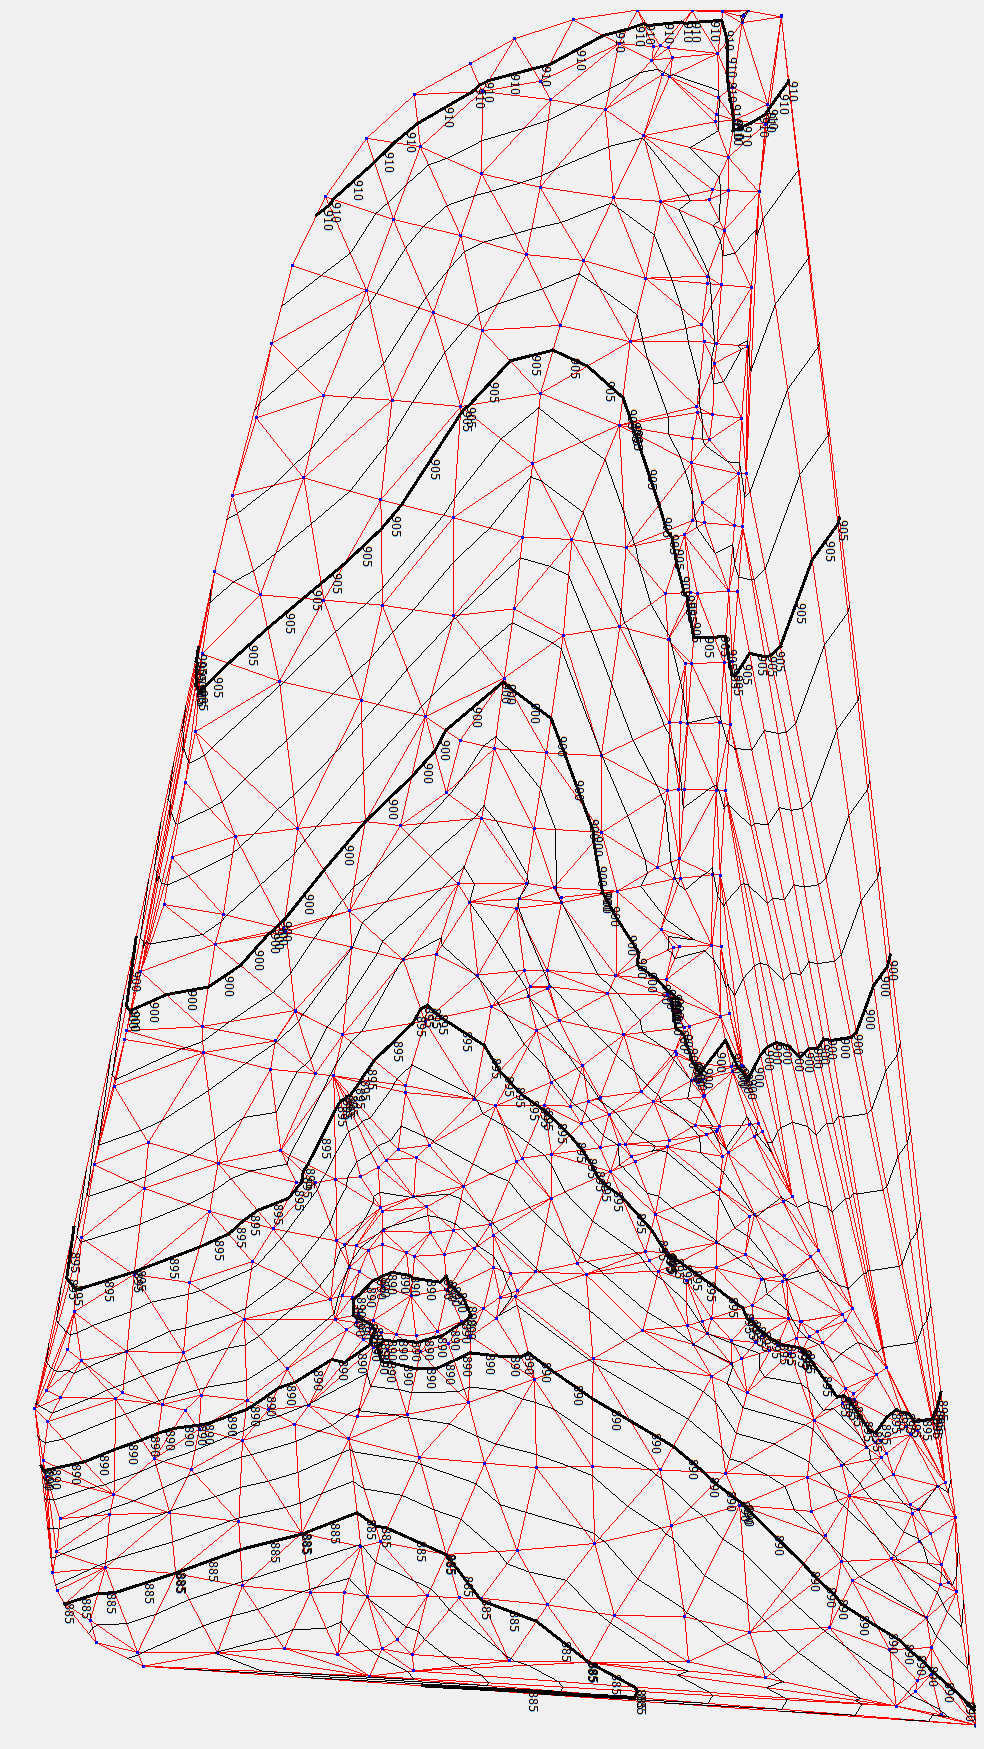
\includegraphics[width=10cm]{DMT_vrstevnice.jpg}
	\caption{Údolnice - vrstevnice}
\end{figure}

\clearpage
\begin{figure}[h]
	\centering
	\includegraphics[width=10cm]{dmt_nas.jpg}
	\caption{Údolnice}
\end{figure}

\begin{figure}[h]
	\centering
	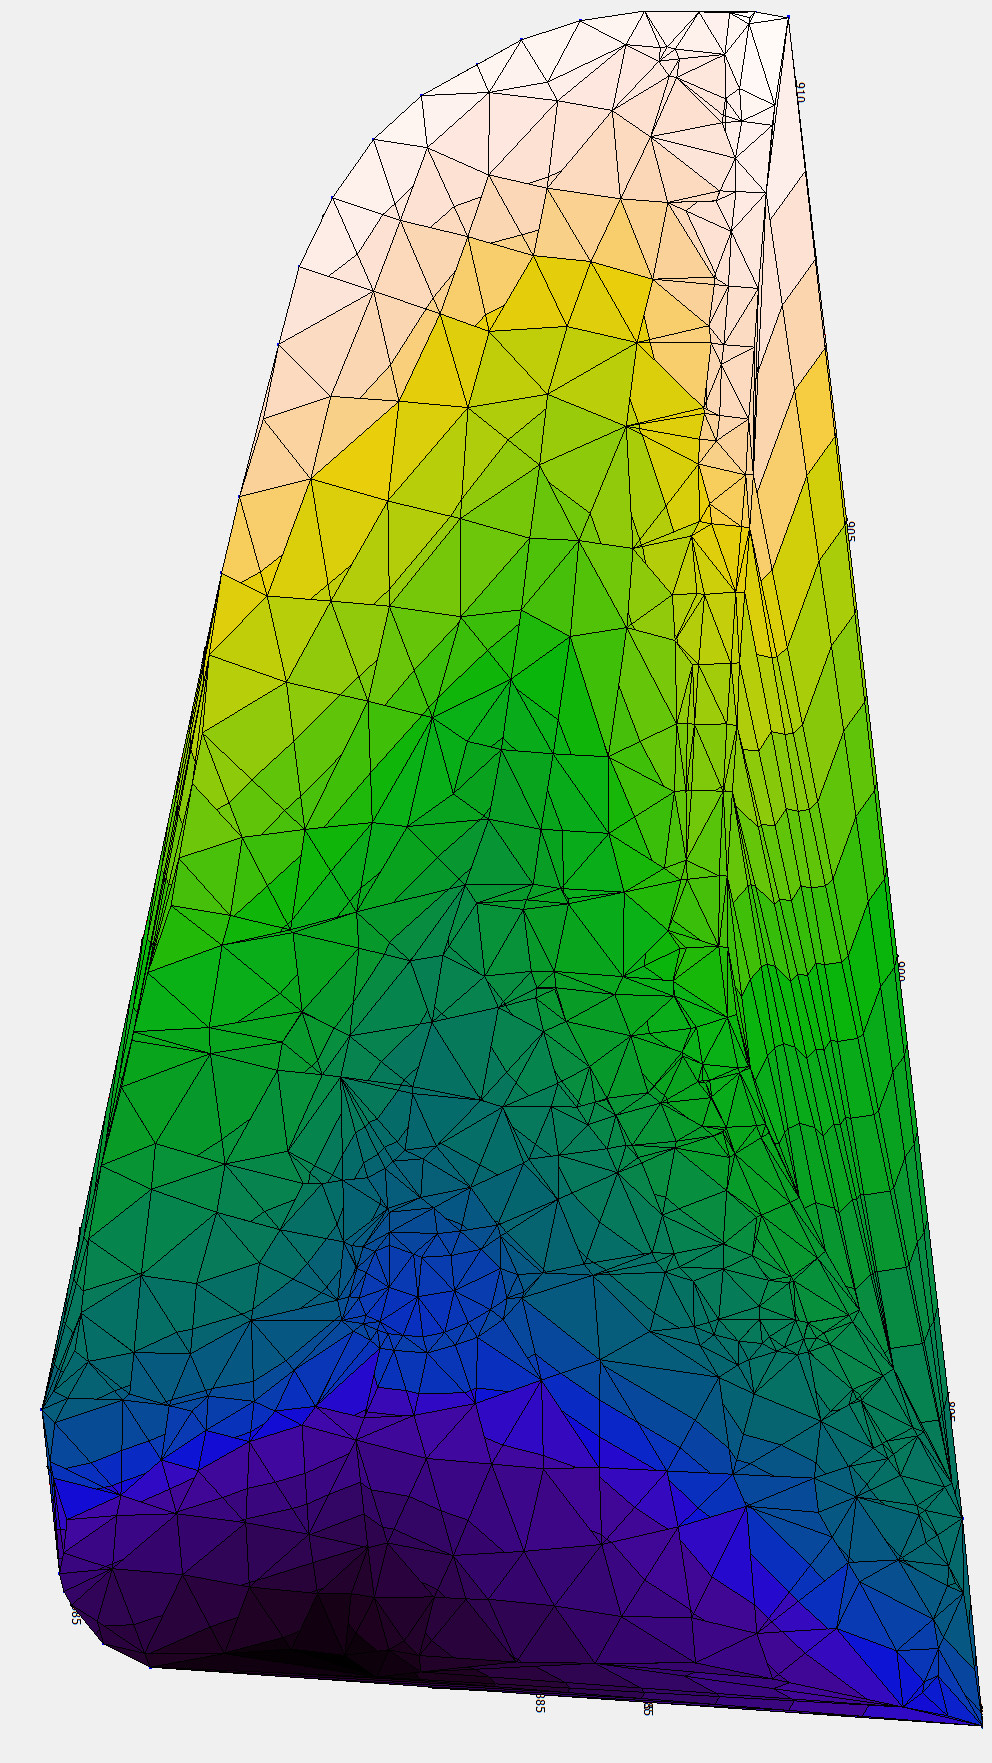
\includegraphics[width=10cm]{DMT_hypsometrie.jpg}
	\caption{Údolnice - hypsometrie}
\end{figure}
\clearpage

\textbf{Celkové zhodnocení}\\

Algoritmus DT není vhodný pro vyjádření terénu, kde jsou ostré hrany - např. chodník, silnice, zídky či ostré terénní hrany, což může být řešeno poloautomatickým zpracováním, kde by se ručně zadaly povinné hrany. Kráter a hřbetnice jsou v kombinaci s vrstevnicemi zobrazeny poměrně obstojně. Algoritmus je zcela vhodný pro území bez výrazných terénních prvků především hran.
\clearpage
%=======================================================================================

\section {Dokumentace}

%
\subsection{QPoint3D}
Definice nového datového typu \textbf{QPoint3D}, který dědí od třídy \textbf{QPointF}. Rozšíření o výškovou souřadnici \textbf{z}. V defaultním konstruktoru jsou nasteveny implicitní hodnoty souřadnic: $[0,0,0]$.
\begin{itemize}
	\item členská proměnná \textbf{double z} - výška bodu
	\item public metody:
	\begin{itemize}
		\item \textbf{getZ} - získání souřadnice z. Návratovým typem je \textbf{double}. 
		\item \textbf{setZ} - uložení hodnoty do členské proměnné z. Návratovým typem je \textbf{void}. 
	\end{itemize}
\end{itemize}
%======================================================
\subsection{QPolygonFZ}
Definice nového datového typu \textbf{QPolygonFZ}, který dědí od třídy \textbf{QPolygonF}. Rozšíření o průměrnou výšku polygonu.
\begin{itemize}
	\item členská proměnná \textbf{double z\_mid} - průměrná výška polygonu
	\item public metody:
	\begin{itemize}
		\item \textbf{getZ} - získání průměrné výšky polygonu. Návratovým typem je \textbf{double}.
		\item \textbf{setZ} - uložení průměrné výšky. Návratovým typem je \textbf{void}.
	\end{itemize}
\end{itemize}

\subsection{Edge}
Definice nového datového typu \textbf{Edge}. Uspořádaná dvojice vrcholů simulující orientovanou hranu (startovní a koncový vrchol).

\begin{itemize}
	\item členské proměnné \textbf{QPoint3D s, e} - počáteční a koncový bod hrany
	\item public metody:
	\begin{itemize}
		\item \textbf{getS resp. getE} - získání počátečního resp. koncového bodu hrany. Návratovým typem je \textbf{QPoint3D}. 
		\item \textbf{switchOr} - metoda slouží ke změně orientace hrany - prohodí počáteční a koncový bod. Návratovým typem je \textbf{void}. 
	\end{itemize}
	\item Přetížení operátoru == pro porovnání dvou hran (hrany se rovnají, pokud mají shodný počáteční a koncový bod).
\end{itemize}

\subsection{Triangle}
%=======================================================
% Doplniš to prosím? Jasan
%======================================================
Definice nového datového typu \textbf{Triangle}. Ukládá trojici vrcholů a sklon a expozici jimi tvořeného trojúhelníku.

\begin{itemize}
	\item členské proměnné:\\ \textbf{QPoint3D p1,p2,p3} - tři vrcholy trojúhelníku \\
	\textbf{double slope, aspect} - sklon a expozice trojúhelníku
	\item public metody \textbf{get$<$}\textit{příslušná členská proměnná}\textbf{$>$} - vrací danou proměnnou.
\end{itemize}

\subsection{Sortovací kritéria}
\begin{itemize}
\item \textbf{SortByXAsc} - řazení bodů typu \textbf{QPoint3D} podle rostoucí souřadnice x, při rovnosti podle y.
\item \textbf{SortByZAsc} - řazení bodů typu \textbf{QPoint3D} podle rostoucí souřadnice z, při rovnosti podle y, při rovnosti podle x.
\item \textbf{SortPolByZAsc} - řazení polygonů typu \textbf{QPolygonFZ} podle střední výšky polygonu.
\end{itemize}


\subsection{Algorithms}
V třídě Algorithms jsou staticky implementovány algoritmy počítající Delaunay triangulaci, vrstevnice, analýzu DMT (sklon a expozici) - a barevnou hypsometrii. 

\begin{itemize}

	\item Výčtový typ \textbf{TPosition}
		\begin{itemize}
			\item Typ využitý jako návratová hodnota členské metody \textbf{getPointLinePosition}.
			\item \textbf{LEFT = 0}
			\item \textbf{RIGHT = 1}
			\item \textbf{ON = 2}
		\end{itemize}

	\item Metoda \textbf{getPointLinePosition}
		\begin{itemize}
			\item Tato metoda slouží k určení polohy bodu vůči přímce. Návratovou hodnotou je výčtový typ \textbf{TPosition}.
			\item Vstup
				\begin{itemize}
					\item \textbf{QPoint3D \&q} - určovaný bod
					\item \textbf{QPoint3D \&a, \&b} - body přímky
				\end{itemize}
			\item Výstup
				\begin{itemize}
					\item \textbf{LEFT} - bod vlevo od přímky
					\item \textbf{RIGHT} - bod vpravo od přímky
					\item \textbf{ON} - bod na přímce
				\end{itemize}

		\end{itemize}


	\item Metoda \textbf{getCircleRadius}
		\begin{itemize}
			\item Tato metoda slouží k výpočtu poloměru opsané kružnice. Návratovou hodnotou je \textbf{double}.
			\item Vstup
				\begin{itemize}
					\item \textbf{QPoint3D \&p1, \&p2, \&p3, \&c} - body $p_i$ definují kružnici, do bodu c jsou ukládány souřadnice středu kružnice.
				\end{itemize}
			\item Výstup
				\begin{itemize}	
					\item Vypočtený poloměr kružnice.
				\end{itemize}
		\end{itemize}	
		
	\item Metoda \textbf{getNearestPoint}		
	\begin{itemize}
		\item Tato metoda slouží k vyhledání nejbližšího bodu. Návratovou hodnotou je \textbf{int}.
		\item Vstup
		\begin{itemize}
			\item \textbf{QPoint3D \&p, std::vector$<$QPoint3D$>$ \&points} - od bodu $p$ je hledán nejbližší bod z vektoru bodů $points$.
		\end{itemize}
		\item Výstup
		\begin{itemize}	
			\item index nejbližšího bodu.
		\end{itemize}
	\end{itemize}	
	
	\item Metoda \textbf{distance}		
	\begin{itemize}
		\item Tato metoda slouží k výpočtu vzdálenosti dvou bodů. Návratovou hodnotou je \textbf{double}.
		\item Vstup
		\begin{itemize}
			\item \textbf{QPoint3D \&p1, QPoint3D \&p2} 
		\end{itemize}
		\item Výstup
		\begin{itemize}	
			\item vzdálenost dvou bodů.
		\end{itemize}
	\end{itemize}

	\item Metoda \textbf{getDelaunayPoint}		
\begin{itemize}
	\item Tato metoda slouží k vyhledání bodu, který vyhovuje kritériím Delaunay triangulace. Návratovým typem je \textbf{int}.
	\item Vstup
	\begin{itemize}
		\item \textbf{QPoint3D \&s, QPoint3D \&e, std::vector$<$QPoint3D$>$ \&points} 
	\end{itemize}
	\item Výstup
	\begin{itemize}	
		\item index bodu.
	\end{itemize}
\end{itemize}

	\item Metoda \textbf{DT}		
\begin{itemize}
	\item Tato metoda slouží k vytvoření vektoru, v němž jsou uloženy hrany Delaunay triangulace. Návratovým typem je \textbf{std::vector$<$Edge$>$ }.
	\item Vstup
	\begin{itemize}
		\item \textbf{std::vector$<$QPoint3D$>$ \&points} 
	\end{itemize}
	\item Výstup
	\begin{itemize}	
		\item vektor hran Delaunay triangulace.
	\end{itemize}
\end{itemize}

	\item Metoda \textbf{getContourPoint}		
\begin{itemize}
	\item Tato metoda slouží k vypočtení souřadnic průsečíku vrstevnice a hrany DT. Návratovým typem je \textbf{QPoint3D}.
	\item Vstup
	\begin{itemize}
		\item \textbf{QPoint3D \&p1,\&p2, double z}, z je výška vrstevnice, bod $p_1$ resp. $p_2$ je počáteční resp. koncový bod hrany.
	\end{itemize}
	\item Výstup
	\begin{itemize}	
		\item průsečík vrstevnice a trojúhelníku DT.
	\end{itemize}
\end{itemize}

	\item Metoda \textbf{createContours}		
\begin{itemize}
	\item Tato metoda slouží k vypočtení vrstevnic a barevné hypsometrie. Návratovým typem je \textbf{std::vector$<$Edge$>$}.
	\item Vstup
	\begin{itemize}
		\item \textbf{std::vector$<$Edge$>$ \&dt} - vektor hran
		\item \textbf{double z\_min, double z\_max, double dz} - rozsah vrstevnic a jejich krok
		\item \textbf{std::vector$<$double$>$ \&contour\_heights} - vektor, do kterého jsou ukládány výšky vrstevnic, pořadí stejné jako pořadí hran vrstevnic ve výstupu z metody
		\item \textbf{std::vector$<$QPolygonFZ$>$ \&hyps} - vektor, do kterého jsou ukládány polygony jednoho intervalu vrstevnic v rámci jednoho trojúhelníku (pro barevnou hypsometrii). 
	\end{itemize}
	\item Výstup
	\begin{itemize}	
		\item vektor hran vrstevnic.
	\end{itemize}
\end{itemize}

	\item Metoda \textbf{getSlope}		
\begin{itemize}
	\item Tato metoda slouží k výpočtu sklonu trojúhelníku. Návratovým typem je \textbf{double}.
	\item Vstup
	\begin{itemize}
		\item \textbf{QPoint3D \&p1, \&p2, \&p3} - vrcholy trojúhelníku.
	\end{itemize}
	\item Výstup
	\begin{itemize}	
		\item sklon trojúhelníku ve stupních.
	\end{itemize}
\end{itemize}

	\item Metoda \textbf{getAspect}		
\begin{itemize}
	\item Tato metoda slouží k výpočtu expozice trojúhelníku. Návratovým typem je \textbf{double}.
	\item Vstup
	\begin{itemize}
		\item \textbf{QPoint3D \&p1, \&p2, \&p3} - vrcholy trojúhelníku.
	\end{itemize}
	\item Výstup
	\begin{itemize}	
		\item expozice trojúhelníku ve stupních.
	\end{itemize}
\end{itemize}

	\item Metoda \textbf{analyzeDMT}		
\begin{itemize}
	\item Tato metoda slouží k vytvoření trojúhelníků a výpočtu jejich sklonu a expozice. Návratovým typem je \textbf{std::vector$<$Triangle$>$}.
	\item Vstup
	\begin{itemize}
		\item \textbf{std::vector$<$Edge$>$ \&dt} - vektor hran Delaunay triangulace.
	\end{itemize}
	\item Výstup
	\begin{itemize}	
		\item vektor trojúhelníků a jejich sklon a expozice.
	\end{itemize}
\end{itemize}

\item Metoda \textbf{processPts}
\begin{itemize}
	\item Tato metoda slouží k vytvoření vektoru polygonů se střední výškou podle zadaného kroku pro barevnou hypsometrii. Návratovým typem je \textbf{void}.
	\item Vstup
	\begin{itemize}
		\item \textbf{std::vector$<$QPoint3D$>$ \&pts} - body, z nichž jsou polygony tvořeny
		\item \textbf{double dz} - krok vrstevnic
		\item \textbf{std::vector$<$QPolygonFZ$>$ \&pols} - vektor, do něhož jsou vytvořené polygony ukládané.
	\end{itemize}
\end{itemize}

	\item Metoda \textbf{sweepLineCH}
\begin{itemize}
	\item Tato metoda slouží k výpočtu konvexní obálky pomocí algoritmu Sweep Line. Jejím výstupním typem je \textbf{QPolygonF}. Metoda použita při výpočtu barevné hypsometrie.
	\item Vstup
	\begin{itemize}
		\item \textbf{std::vector} $<$\textbf{QPointF}$>$ \textbf{\&points} - vektor bodů, kolem nichž má být vytvořená konvexní obálka.
	\end{itemize}
	\item Výstup
	\begin{itemize}
		\item Polygon obsahující konvexní obálku.
	\end{itemize} 
\end{itemize}

\item Metoda \textbf{avgH}
\begin{itemize}
	\item Metoda slouží k výpočtu průměrné výšky zadaných bodů. Návratovým typem je \textbf{double}.
	\item Vstup - \textbf{std::vector$<$QPoint3D$>$ \&pts} - vstupní body
	\item Výstup - průměrná hodnota výšek
	
\end{itemize}

\end{itemize}	


\subsection{Draw}
Třída draw slouží k vykreslení načtených bodů, vypočtené Delaunay triangulace, vrstevnic, sklonu, expozice a hypsometrie. Třída dědí od třídy \textbf{QWidget}. 

\begin{itemize}
	\item Členské proměnné
		\begin{itemize}
			\item \textbf{std::vector $<$QPoint3D$>$ points } vektor načtených bodů
			\item \textbf{std::vector $<$Edge$>$ dt }- vektor hran Delaunay triangulace
			\item \textbf{std::vector $<$Edge$>$ contours} - vektor hran vrstevnic
			\item \textbf{std::vector $<$double$>$ contours\_heights} - vektor výšek vrstevnic
			\item \textbf{std::vector $<$Triangle$>$ dtm} - vektor trojúhelníků Delaunay triangulace
			\item \textbf{std::vector $<$QPolygonFZ$>$ hyps} - vektor polygonů hypsometrie
			\item \textbf{int step} - rozestup vrstevnic
			\item \textbf{bool draw\_main} - flag vykreslení hlavních vrstevnic
			\item \textbf{bool draw\_slope} - flag vykreslení sklonu - v konstruktoru třídy nastaveno na false
			\item \textbf{bool draw\_aspect} - flag vykreslení expozice - v konstruktoru třídy nastaveno na false
			\item \textbf{bool draw\_hyps} - flag vykreslení barevné hypsometrie - v konstruktoru třídy nastaveno na false
			\item \textbf{std::vector $<$QColor$>$ ctable} - tabulka barev pro hypsometrii, v konstruktoru třídy načtena ze souboru
		\end{itemize}
	
	\begin{itemize}
	\item Metoda \textbf{paintEvent}
		\begin{itemize}
			\item Tato metoda slouží k vykreslení načtených bodů, vypočtené Delaunay triangulace, vrstevnic, sklonu, expozice a hypsometrie. Metoda se volá pomocí metody \textbf{repaint()}. Návratovým typem je \textbf{void}.
			\item Vstup
				\begin{itemize}
					\item \textbf{QPaintEvent *e}
				\end{itemize}
		\end{itemize}

%	\item Metoda \textbf{mousePressEvent}
%		\begin{itemize}
%			\item Metoda sloužící k uložení bodu do členské proměnné \textbf{points} určeného kliknutím myší nad kreslícím plátnem. Jejím návratovým typem je \textbf{void}.	
%			\item Vstup
%				\begin{itemize}
%					\item \textbf{QMouseEvent *e}
%				\end{itemize}
%		\end{itemize}

\item Metoda \textbf{clearPoints}
		\begin{itemize}
			\item Tato metoda slouží pro vymazání bodů.
		\end{itemize}	

	\item Metoda \textbf{clearDT}
		\begin{itemize}
			\item Tato metoda slouží pro vymazání bodů, triangulace, vrstevnic a hypsometrie. Na vstupu není nic a je typu void.
		\end{itemize}	

	\item Metoda \textbf{getPoints}
Tato metoda vrací členskou proměnnou \textbf{std::vector $<$QPoint3D$>$ points}.


	\item Metoda \textbf{getDT}
Tato metoda vrací členskou proměnnou \textbf{std::vector $<$Edge$>$ dt }.
%=======================================================================================================
	\item Metoda \textbf{setDT}
Tato metoda slouží k přiřazení hodnot členské proměnné dt.

	\item Metoda \textbf{setContours}
Metoda slouží k přiřazení hodnot členským proměnným \textbf{std::vector $<$Edge$>$ contours}, \textbf{std::vector $<$double$>$ contours\_heights}, \textbf{int step}, \textbf{bool draw\_main} a \textbf{std::vector $<$QPolygonFZ$>$ hyps}.

\item Metoda \textbf{setDTM}
Tato metoda slouží k přiřazení hodnot členské proměnné \textbf{std::vector $<$Triangle$>$ dtm}.

	\item Metoda \textbf{loadPoints}
\begin{itemize}
	\item Tato metoda slouží pro načtení bodů z textového souboru do vektoru \textbf{points} a pro určení minimální a maximální výšky bodů v souboru. Zároveň je zvoleno "měřítko" kanvasu dle velikosti kanvasu a rozsahu vstupních dat. Návratovým typem je \textbf{void}.
	\item Vstup
	\begin{itemize}
		\item \textbf{std::string points\_path} - cesta k vstupnímu souboru
		\item \textbf{QSizeF \&canvas\_size} - velikost kanvasu
		\item \textbf{double \&min\_z, \&max\_z} - nejmenší/největší výška
	\end{itemize}
\end{itemize}
%=======================================================
%Tady nevím, jak to napsat, doplniš to prosím? oujé
%======================================================
	\item Metoda \textbf{setDrawSlope}
	\begin{itemize}
		\item Tato metoda slouží k zapnutí/vypnutí vykreslování sklonu a k vypnutí vykreslování expozice a hypsometrie. 
	\end{itemize}
%
%
	\item Metoda \textbf{setDrawAspect}
	\begin{itemize}
		\item Tato metoda slouží k zapnutí/vypnutí vykreslování expozice a k vypnutí vykreslování sklonu a hypsometrie. 
	\end{itemize}

\item Metoda \textbf{drawHypsometry}
\begin{itemize}
		\item Tato metoda slouží k zapnutí/vypnutí vykreslování hypsometrie a k vypnutí vykreslování sklonu a expozice. 
	\end{itemize}
%========================================================
	
	\item Metoda \textbf{genAspColor}
	\begin{itemize}
	\item Metoda slouží k nastavení barev pro expozici. Jejím návratovým typem je \textbf{std::vector$<$QColor$>$}. Na vstupu nemá nic, vrací vektor barev.
	\end{itemize}

%	


\end{itemize}
\end{itemize}



\clearpage


\subsection{Widget}
Tato třída slouží ke komunikaci s GUI. Třída dědí od třídy QWidget. Všechny její metody slouží jako sloty k signálům z GUI, nemají žádné vstupní hodnoty a jejich návratovým typem je void. 

\begin{itemize}
	
	\item Členské proměnné \textbf{double z\_min, double z\_max} - instance třídy si drží minimální a maximální výšku vstupních bodů

	\item Metoda \textbf{on\_trg\_button\_clicked} - výpočet triangulace a její vizualizace.

	\item Metoda \textbf{on\_clear\_button\_clicked} - maže obsah kanvasu.
	
	\item Metoda \textbf{on\_cont\_button\_clicked} - výpočet vrstevnic a hypsometrie, vizualizace vrstevnic.

	\item Metoda \textbf{on\_slope\_button\_clicked} - výpočet a vizualizace sklonu. 

	\item Metoda \textbf{on\_load\_points\_button\_clicked} - načtení a vizualizace vstupních bodů. Nastavení minimální a maximální výšky vstupních bodů do členských proměnných.
	
	\item Metoda \textbf{on\_aspect\_button\_clicked} - výpočet a vizualizace expozice.
	
	\item Metoda \textbf{on\_hyps\_button\_clicked} - vizualizace barevné hypsometrie.

\end{itemize} 


\clearpage

\section{Přílohy}

\begin{itemize}
	\item Příloha č.1: Testovací data - \textit{testovaci\_data.txt}.
	\item Příloha č.2: Testovací data pro různé terénní prvky - \textit{testovaci\_data2.txt}.
\end{itemize}
 %--------------------------------------------------------------------------------------------------------------------------------------------------------------------------
\clearpage
\section{Závěr}

\subsection{Zhodnocení}
Implementace barevné hypsometrie by šla\begin{flushright}
	\begin{flushright}
		
	\end{flushright}
\end{flushright} provést určitě lépe a efektivněji, nicméně s naším postupem jsme spokojeni, protože jsme si ho vymysleli sami. To, že implementace zabrala hodně času (zvlášť ladění) a asi o hodně víc času (hloupé chyby -$>$ debugování (debeatlesování?) levelu Yoko Ono) než nepovinné úlohy za dvojnásobek bodů (resp. ta s generováním terénních útvarů), nám nevadí, protože jedeme spíš na to, co nás baví a barvičky baví každého.
\subsection{Návrhy na vylepšení}
Nynější automatické popisky vrstevnic jsou spíš ošklivé než hezké, přestože plní účel. Popisky by tedy chtělo vylepšit, aby respektovaly kartografické zásady. Dále by také bylo vhodné přizpůsobit vizualizaci sklonu dle rozsahu sklonů ve zpracovávaných datech a možná by stála za to změna barevné mapy při vykreslování expozice. Expozice (i když barvy jsou přebrané od ESRI) není takto moc intuitivní. 

\clearpage
\section{Zdroje}

\begin{enumerate}
\item  BAYER, Tomáš. 2D triangulace, DMT [online][cit. 1.12.2018]. \\
Dostupné z: https://web.natur.cuni.cz/~bayertom/images/courses/Adk/adk5.pdf  \\

\item  BAYER, Tomáš. 2D triangulace, DMT [online][cit. 30.11.2018]. \\
Dostupné z: https://web.natur.cuni.cz/~bayertom/images/courses/Adk/adkcv3.pdf\\

\item Tools: Aspect. ArcMap|ArcGIS Desktop [online]. Environmental Systems Research Institute, 2016 [cit. 2018-12-02]. \\
Dostupné z: http://desktop.arcgis.com/en/arcmap/10.3/tools/spatial-analyst-toolbox/how-aspect-works.htm\\
%=======================================================================================
\end{enumerate}

\end{document}



 
